\newpage
\chapter{Similar-sized collisions: A parameter study}
\graphicspath{{./03figs/}}
In cratering collisions, where the impactor is much smaller than the target, the impactor hits the target completely and is fully stopped. The critical impact angle for which only half the impactor volume is being hit is roughly
\begin{equation}
\label{ch03_eq001}
\cos{ \theta_{graz} }= \frac{\Rtar}{\Rtar + \Rimp}
\end{equation}

One can directly see that for cratering collisions where $\Rimp \ll \Rtar$ this angle is nearly $90^\circ$ and the impactor is efficiently stopped for $\thimp < \theta_{graz}$. Figure \label{ch03_fig03} shows on the right side an illustration of $\theta_{graz}$. Such cratering collisions can be reduced to a point source of energy, comparable to an explosion \citep{Melosh:2007p3502}. Scaling laws exist for the resulting crater depth and shape \citep{Holsapple:1993p3018}.
\begin{figure}[htbp]
\begin{center}
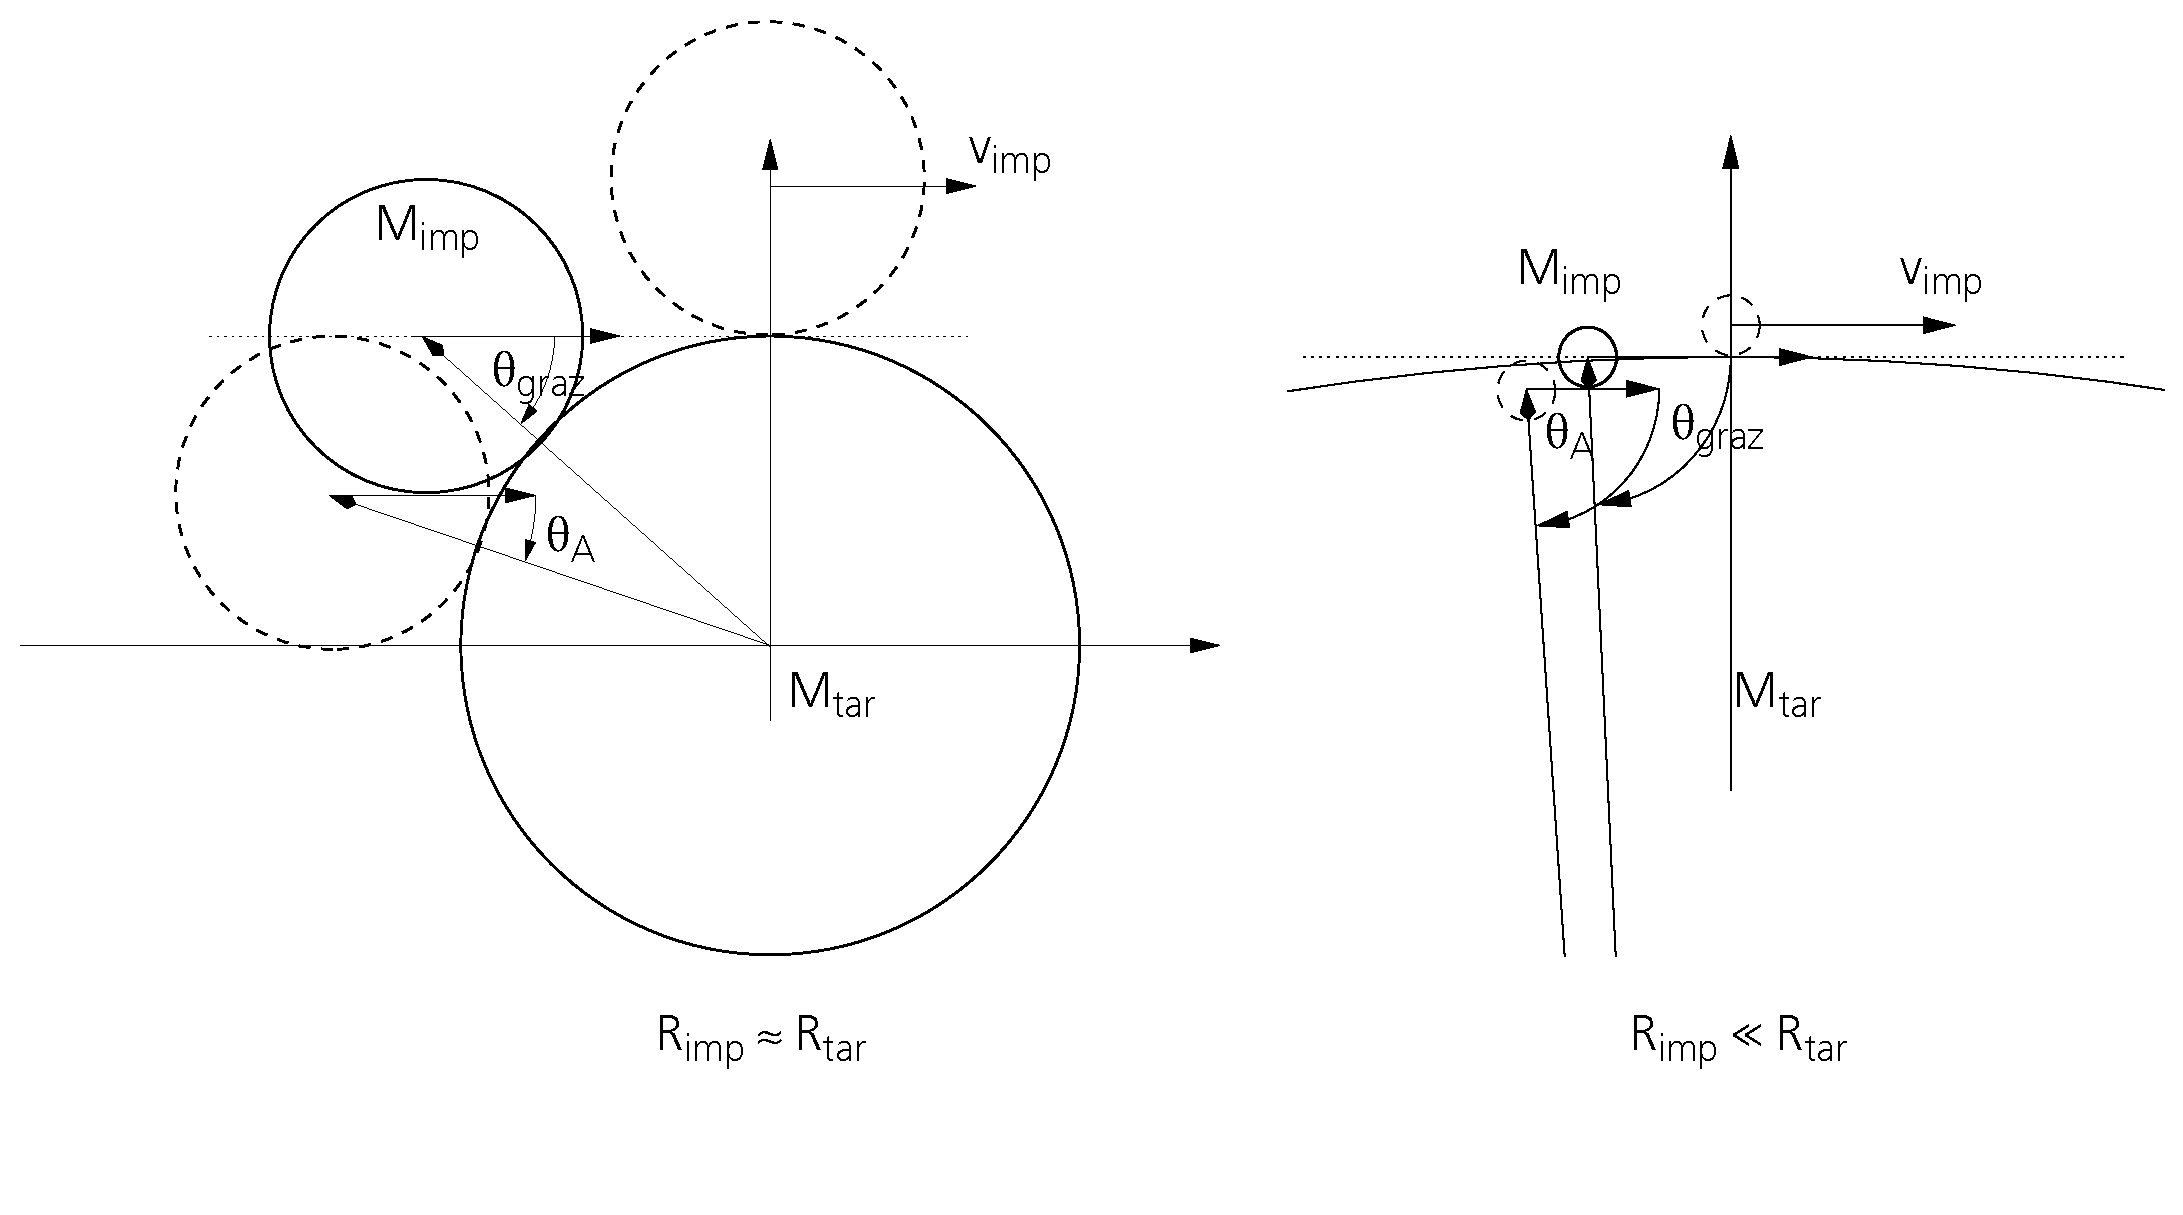
\includegraphics[scale=0.4]{03_grazing}
\caption{Impact geometry for a \SSC on the left side. The right plot shows a collision between a relatively small impactor compared to the target. The grazing impact angle $\theta_{graz}$ is defined as the angle for which half of the impactor simply grazes past the target \citep{Asphaug:2010p3539}. The dashed circles show the largest impact angle for which no impactor material would graze past the target $\theta_A$ and the $90^\circ$ impact angle for which the whole impactor grazes past the target. Note }
\label{ch03_fig03}
\end{center}
\end{figure}

In similar-sized collisions, where the target has a mass in the same order of magnitude as the impactor, the collision becomes more complex. Whilst being stopped, the target itself is altered and parts of the impactor miss the target completely depending on the impact angle. The left part of figure \label{ch03_fig03} shows an example of a similar-sized collision for which $\theta_{graz} \approx 45^\circ$. Assuming the impactor follows a straight trajectory and is not tidally deformed, the relative volume of either the impactor hitting the target $V_{hit, imp}$ or vice versa $V_{hit, tar}$, can be calculated numerically (see appendix section \label{ch07_sec01}). Figure shows these two variables as a function of $\gamma = \Mimp / \Mtar$ and the impact angle.
\begin{figure}[htbp]
\begin{center}
\includegraphics[scale=0.7]{05_Mhit}
\caption{Relative volume of the impactor ($V_{hit, imp}$, left plots) and the target ($V_{hit, tar}$, right plots) hit by the other body as a function of impact angle (top plots) and impact parameter (bottom plots) for different mass ratios $\gamma$. Compare figure \ref{ch07_fig01} for an illustration of those volumes. Note that the ratio of radii scales with the cubic root of the mass ratio: $R_{imp} / R_{tar} \sim \sqrt[3]{\gamma}$. The dotted line shows for which impact angle half of the impactor volume grazes past the target. } 
\label{ch03_fig05}
\end{center}
\end{figure}

Whilst for a small $\gamma$ the function becomes a step function with a sharp drop-off at $90^\circ$, already for a $\gamma = 0.1$, the relative volume hit by the impactor varies between 0 and 1 over an impact angle range of $30^\circ$. 


The target is altered on it entire scale and the outcome of the collision depends on the geometry of the 

The target is only altered on a scale a few times bigger than the impactor. In a similar-sized collision (\SSC), craters 

%Similar-sized collision ( \SSC ) distinct themselves in the break down of certain simplifying aspects of cratering impacts, where the 


Similar sized collisions are a complex process involving gravity, hydro- and thermodynamics and lead to non-trivial post-collision outcomes. This chapters shows the results of a small parameter study, which analyses various interesting parameters which describe those collision outcomes.


The first section gives a quick overview of the physical processes involved in similar sized collisions and their associated timescales.

In a second section, the detailed setup of the simulations and the used parameters are described.

The actual results are presented in the third and discussed in the fourth section.








\section{Introduction}
motivation: moon formation, Lisse stuff, disks \& moons, importance for simulations of terrestrial planet and giant planet core formation, no big study before \\
small impactor: size of impactor vs. central body field gradient small -> almost no torques \\
define grazing angle for each mass ratio (radii ratio) \\
why are SSC non-trivial? \\
lot of spill-over for similar sizes \\
target gets changed \\
Section \ref{ch07_sec01} in the appendix hababa \\


\section{Collision physics}
compare timescales\\
viscous timescale $t = R^2 / \nu$ \\
collisional timescale $t = 2 R / \vimp$ \\
self-gravitational timescale $t = \sqrt{3\pi / G \rho}$ \\
orbital time scale in solar system \\
local gravity, free fall time \\
impact vs. shock velocity (super-sonic), shock waves $t = R / c_S $ \\
surface tension (Walker and Mullins 1981) vs. shearing forces, approximation of fluid bodies \\
compare central potential of a planetary system with local gravity, compare timescales \\
%TODOPLOT: show phenomena in the angle vs. vimp plot
basic process of cratering collisions: contact and compression stage, excavation stage \cite{Melosh:2007p3502} \\


\section{Setup and parameters used}
describe parameter space: fixed target mass and mass ratio, then vary relative impact velocity and impact angle. hit\&run are not considered. \\
how long a simulation is integrated \\
problems: 
post-processing \\
r3, c1, i1 \\
resolution, number of particles, particles per body diameter \\
initial temperature not important, show profiles nevertheless \\

as shown in \ref{ch02_sec04_ss02} and \label{ch02_sec04_ss04}



impact angle of $30\deg$



\begin{figure}[htbp]
\begin{center}
\includegraphics[scale=0.7]{01_overview_params.pdf}
\caption{Impact geometry for a \SSC on the left side. The right plot shows a collision between a relatively small impactor compared to the target. The grazing impact angle $\theta_{graz}$ is defined as the angle for which half of the impactor simply grazes past the target \citep{Asphaug:2010p3539}. The dashed circles show the largest impact angle for which no impactor material would graze past the target $\theta_A$ and the $90^\circ$ impact angle for which the whole impactor grazes past the target. Note }
\label{ch03_fig01}
\end{center}
\end{figure}

\begin{figure}[htbp]
\begin{center}
\includegraphics[scale=0.8]{07_strucs.pdf}
\caption{Isentropic internal structures of the bodies used in the simulations. The first row of plots shows the density profiles, the second row the pressure and the third row the temperatures. The first column of plots shows silicate bodies with a $100 wt\%$ $\silc$ composition with the following masses from left to right: 0.1 (blue curve), 0.2 (red), 0.5 $\ME$ (magenta). The second column shows structures of differentiated bodies of chondritic composition with a $70 wt\%$ $\silc$ mantle and a $30 wt\%$ iron core: 0.002 (red), 0.007 (green), 0.01 (blue), 0.02 (red), 0.035 (black), 0.07 (green), 0.01 (blue), 0.2 (red), 0.7 (green) and 1.0 $\ME$ (blue). The last column on the right shows a few structures with a composition typical to regions beyond the snow line with $50 wt\%$ water ice, $35 wt\%$ $\silc$ and $15 wt\%$ iron. Masses range from 0.002 (red), 0.01 (blue), 0.02 (red), 0.1 (blue), 0.2 (red) and 1.0 $\ME$ (blue) from left to right. The radius of the structures depends on the average density and therefore also on the composition of the bodies. Icy bodies have low average densities compared to chondritic bodies. Note that the bodies entirely composed of $\silc$ have a higher average density than equally massive bodies with a chondritic composition, due to the higher compressibility of $\silc$ compared to iron. In the core of the pure silicate bodies, the density reached more than twice the reference density of $\silc$, while the iron cores of the chondritic bodies is only slightly compressed.}
\label{ch03_fig07}
\end{center}
\end{figure}



% TODOPLOT: insert a summary.pdf example

\section{Results}

%%
% Largest remnant
%% 
\subsection{Largest remnant mass, accretion efficiency $\xi$ and $Q_D$}
compare with previous work\\
\cite{Benz:1988p3336} 0.1 Mearth target, 1:6 mass ratio, vimp = 2.5-8 vesc, all eroding\\
\cite{Benz1999Icar..142....5B}: MLR / Mtarg ~ Q / Q*, parabolic fit \\
\cite{Agnor:2004p3329}  two 0.1Mearth mass bodies, chondritic, Tillotson \\
\cite{Stewart:2009p3265} catastrophic disruption criteria, Mlr / Mtarg replaced by Mlr / Mtot, Q* scaled to reduced mass in kinetic energy \\ 
\cite{2010ApJ...714L..21K} ,mass ratios: 1.0, 0.66, 0.50, 0.33, 0.25, 0.17, 0.11, Mtot = 0.2-2.0MEarth, defined $v_{cr}$ \\
try volumetric scaling for oblique impacts \\
show 4 main categories: accretion, partial accretion, erosion and hit \& run \\
check Benz 1999, Angor \& Asphaug 2004, Stewart \& Leinhardt 2009, Marcus 2009, Marcus 2010 \\
volumetric scaling (Canup 2005, Leinhardt) \\
mention problems with slow accretion producing secondary impacts, show example with very large timescales, problem to estimate result due to pre-rotation\\

\begin{landscape}
\begin{figure}[htbp]
\begin{center}
\includegraphics[scale=1.0]{08_accreff_r3.pdf}
\caption{Accretion efficiency $\xi$ as a function of the impact angle for different relative impact velocities. Each subplot shows a set of simulations for a given target mass $\Mtar$ and mass ratio $\gamma = \Mimp / \Mtar$. Each point shows the outcome of an individual simulation of the \emph{r3} simulation set involving bodies composed purely of $\silc$. The black dashed line shows the relative volume of the impactor hitting the target for the given mass ratio (compare figure \ref{ch03_fig05}).}
\label{ch03_fig08a}
\end{center}
\end{figure}

\begin{figure}[htbp]
\begin{center}
\includegraphics[scale=1.0]{08_accreff_c1.pdf}
\caption{Accretion efficiency $\xi$ for the \emph{r3} simulation set with bodies of chondritic composition (compare figure \ref{ch03_fig08a}. Each row shows a different magnitude of target mass, each column a different mass ratio.}
\label{ch03_fig08b}
\end{center}
\end{figure}

\begin{figure}[htbp]
\begin{center}
\includegraphics[scale=1.0]{08_accreff_i1.pdf}
\caption{Accretion efficiency $\xi$ for the \emph{i1} simulation set with bodies of icy composition (compare figure \ref{ch03_fig08b}).}
\label{ch03_fig08c}
\end{center}
\end{figure}

\begin{figure}[htbp]
\begin{center}
\includegraphics[scale=1.0]{09_accreff_vimp_r3.pdf}
\caption{Accretion efficiency $\xi$ for the \emph{r3} simulation set as a function of impact velocity $\vimp$ for different impact angles. The vertical lines shows the predicted values from \cite{2010ApJ...714L..21K} for the critical impact velocity $v_{cr}$, where accretion changes to erosion and the accretion efficiency goes to negative values.}
\label{ch03_fig09a}
\end{center}
\end{figure}

\begin{figure}[htbp]
\begin{center}
\includegraphics[scale=1.0]{09_accreff_vimp_c1.pdf}
\caption{Accretion efficiency $\xi$ as a function of impact velocity $\vimp$ for different impact angles as in figure \ref{ch03_fig09a} for the \emph{c1} simulation set.}
\label{ch03_fig09b}
\end{center}
\end{figure}

\begin{figure}[htbp]
\begin{center}
\includegraphics[scale=1.0]{09_accreff_vimp_i1.pdf}
\caption{Accretion efficiency $\xi$ as a function of impact velocity $\vimp$ for different impact angles as in figure \ref{ch03_fig09a} for the \emph{i1} simulation set.}
\label{ch03_fig09c}
\end{center}
\end{figure}

\begin{figure}[htbp]
\begin{center}
\includegraphics[scale=1.0]{15_QQRD_r3.pdf}
\caption{Scaled largest remnant masses $M_{LR} / M_{tot}$ as a function of the relative specific impact energy $Q_R / Q^*_{RD}$ as defined in \cite{Stewart:2009p3265} and using the parameters for $Q^*_{RD}$ as in \cite{2010ApJ...712L..73M}. The coloured lines solid lines show the simulation values for the \emph{r3} simulation set and the dashed black line shows the predicted value from the scaling law.}
\label{ch03_fig15a}
\end{center}
\end{figure}

\begin{figure}[htbp]
\begin{center}
\includegraphics[scale=1.0]{15_QQRD_c1.pdf}
\caption{Scaled largest remnant masses $M_{LR} / M_{tot}$ as a function of the relative specific impact energy $Q_R / Q^*_{RD}$ as in figure \ref{ch03_fig15a}, but for the \emph{c1} simulation set.}
\label{ch03_fig15b}
\end{center}
\end{figure}

\begin{figure}[htbp]
\begin{center}
\includegraphics[scale=1.0]{15_QQRD_i1.pdf}
\caption{Scaled largest remnant masses $M_{LR} / M_{tot}$ as a function of the relative specific impact energy $Q_R / Q^*_{RD}$ as in figure \ref{ch03_fig15a}, but for the \emph{i1} simulation set.}
\label{ch03_fig15c}
\end{center}
\end{figure}
\end{landscape}




%%
% secondary remnants 
%% 
\subsection{secondary remnants}
\cite{Agnor:2004p3329} compare with figure 2\\
% TODOPLOT: plot all mass not in largest or second remants compared to total mass

%%
% rotation stuff
%% 
\subsection{Spin-up, critical angular momentum}
\cite{Canup:2000p3542}: critical ang. momentum\\
critical T / W \\
how to get from Erot and I to a rotation rate:
\begin{equation}
T = 2 \pi \sqrt{ \frac{I}{2 E_{rot}} }
\end{equation}
shedding of material due to rotational ejection \\
$L_{bound}$ vs. $L_{imp}$ \\
$t = \frac{T}{|W|}$
$t_{crit} = 0.2738$ for McLaurin spheroids \citep{1987gady.book.....B} \citep{chandrasekhar1969ellipsoidal}

\begin{landscape}
\begin{figure}[htbp]
\begin{center}
\includegraphics[scale=1.0]{19_rotperiod_c1.pdf}
\caption{Rotation period of the largest remnant as a function of impact angle for the \emph{r3} simulation set. Only particles in the remnant are considered which are part of the largest clump and not in a disk orbit. Solid body rotation is assumed for calculating the rotation period by simply comparing the rotational energy with the moment of intertia: $T = 2 \pi \frac{I}{2 E_{rot}}$.}
\label{ch03_fig19a}
\end{center}
\end{figure}

\begin{figure}[htbp]
\begin{center}
\includegraphics[scale=1.0]{10_rotstab_c1.pdf}
\caption{Dimensionless rotational stability parameter $t = \frac{T}{|W|}$ comparing the rotational energy $T$ with the potential energy $W$ for the largest remnant in the \emph{r3} simulation set. Note that again only particles from the actual clump are considered for calculating both energies. Disk particles are not considered.}
\label{ch03_fig10a}
\end{center}
\end{figure}

\begin{figure}[htbp]
\begin{center}
\includegraphics[scale=1.0]{19_rotperiod_c1.pdf}
\caption{Rotation period of the largest remnant as a function of impact angle for the \emph{c1} simulation set as in figure \ref{ch03_fig19a} }
\label{ch03_fig19b}
\end{center}
\end{figure}

\begin{figure}[htbp]
\begin{center}
\includegraphics[scale=1.0]{10_rotstab_c1.pdf}
\caption{Dimensionless rotational stability parameter $t = \frac{T}{|W|}$ for the largest remnant as a function of impact angle as in figure \ref{ch03_fig10a} but for simulation set \emph{c1}.}
\label{ch03_fig10b} 
\end{center}
\end{figure}

\begin{figure}[htbp]
\begin{center}
\includegraphics[scale=1.0]{19_rotperiod_i1.pdf}
\caption{Rotation period of the largest remnant as a function of impact angle for the \emph{i1} simulation set as in figure \ref{ch03_fig19a} }
\label{ch03_fig19c}
\end{center}
\end{figure}

\begin{figure}[htbp]
\begin{center}
\includegraphics[scale=1.0]{10_rotstab_i1.pdf}
\caption{Dimensionless rotational stability parameter $t = \frac{T}{|W|}$ for the largest remnant as a function of impact angle as in figure \ref{ch03_fig10a} but for simulation set \emph{i1}.}
\label{ch03_fig10c}
\end{center}
\end{figure}
\end{landscape}



%%
% energy partition
%% 
\subsection{Energy partition}
potential, internal and rotational energy\\
energy partition in bodies (shocks, tidal vs. self-gravity stress) \\
$\Delta U$, accretion vs. non-accretion \\


\begin{landscape}
\begin{figure}[htbp]
\begin{center}
\includegraphics[scale=1.0]{11_dU_impa_r3.pdf}
\caption{Change in internal energy $\Delta U$ relative to the impact energy $E_{imp} = \frac{1}{2}\mu \vimp$ for the largest remnant as a function of the impact angle for the simulation set \emph{r3}.}
\label{ch03_fig11a}
\end{center}
\end{figure}

\begin{figure}[htbp]
\begin{center}
\includegraphics[scale=1.0]{11_dU_impa_c1.pdf}
\caption{Change in internal energy $\Delta U$ as in figure \ref{ch03_fig11a}, but for the simulation set \emph{c1}.}
\label{ch03_fig11b}
\end{center}
\end{figure}

\begin{figure}[htbp]
\begin{center}
\includegraphics[scale=1.0]{11_dU_impa_i1.pdf}
\caption{Change in internal energy $\Delta U$ as in figure \ref{ch03_fig11a}, but for the simulation set \emph{i1}.}
\label{ch03_fig11c}
\end{center}
\end{figure}

\begin{figure}[htbp]
\begin{center}
\includegraphics[scale=1.0]{12_dPot_impa_r3.pdf}
\caption{Change in potential energy $\Delta W$ relative to the impact energy $E_{imp} = \frac{1}{2}\mu \vimp$ for the largest remnant as a function of the impact angle for the simulation set \emph{r3}.}
\label{ch03_fig12a}
\end{center}
\end{figure}

\begin{figure}[htbp]
\begin{center}
\includegraphics[scale=1.0]{12_dPot_impa_c1.pdf}
\caption{Change in potential energy $\Delta W$ as in figure \ref{ch03_fig12a}, but for the simulation set \emph{c1}.}
\label{ch03_fig12b}
\end{center}
\end{figure}

\begin{figure}[htbp]
\begin{center}
\includegraphics[scale=1.0]{12_dPot_impa_i1.pdf}
\caption{Change in potential energy $\Delta W$ as in figure \ref{ch03_fig12a}, but for the simulation set \emph{i1}.}
\label{ch03_fig12c}
\end{center}
\end{figure}
\end{landscape}



%%
% compositional changes
%% 
\subsection{Compositional changes, mixing}
mainly for next largest bodies\\
mantle striping\\
impactor perspective\\
accr. efficiencies for individual components \\
compositional changes for h\&r \\
introduce alternative impact angles $\theta_{core}$ \\
give volumetric estimate \\
compare sound speed with impact velocity to check for shocking (vimp vs. vsound), define vimprel which becomes supersonic \\

\begin{equation}
\delta_X = \frac{M_{SR} - M_{imp}}{M_{imp}} \Bigg|_{X}
\end{equation}

\begin{landscape}
\begin{figure}[htbp]
\begin{center}
\includegraphics[scale=1.0]{18_strpeff_vimp_c1.pdf}
\caption{Difference of striping efficiency for silicate and iron ($\delta_{\silc} - \delta_{Fe}$) as a function of impact angle for the \emph{c1} simulation set.}
\label{ch03_fig18a}
\end{center}
\end{figure}

\begin{figure}[htbp]
\begin{center}
\includegraphics[scale=1.0]{18_strpeff_vimp_i1.pdf}
\caption{DIfference of striping efficiency for silicate and iron ($\delta_{\silc} - \delta_{Fe}$) and for water ice and silicate ($\delta_{H_2 O} - \delta_{\silc}$) as a function of impact angle for the \emph{i1} simulation set.}
\label{ch03_fig19a}
\end{center}
\end{figure}

\begin{figure}[htbp]
\begin{center}
\includegraphics[scale=1.0]{23_impa_vs_corea_c1.pdf}
\caption{The impact angle of the impactors iron core against the targets iron core $\theta_{Fe}$ as a function of actual impact angle $\thimp$ of the bodies for the \emph{c1} simulation set.}
\label{ch03_fig23a}
\end{center}
\end{figure}

\begin{figure}[htbp]
\begin{center}
\includegraphics[scale=1.0]{23_impa_vs_corea_i1.pdf}
\caption{The impact angle of the impactors iron core against the targets iron core $\theta_{Fe}$ and the silicate layers of the two bodies $\theta_{\silc}$ as a function of actual impact angle $\thimp$ of the bodies for the \emph{i1} simulation set.}
\label{ch03_fig23b}
\end{center}
\end{figure}
\end{landscape}




%%
% disk formation
%% 
\subsection{Satellite and disk formation}
crucial for life? (Laskar paper, E)\\
analyze disk masses, angular momentum \& composition \\
mean a and mean e, compare with roche limit \\
satellite formation in second \\

\begin{landscape}
\begin{figure}
\begin{center}
\includegraphics[scale=1.0]{13_mdisk_impa_r3.pdf}
\caption{Largest remnant total disk mass as a function of impact angle for different impact velocities for the \emph{r3} simulation set. Simulations with a largest remnant disk mass below $0.1\% M_{tot}$ are omitted.}
\label{ch03_fig13a}
\end{center}
\end{figure}

\begin{figure}
\begin{center}
\includegraphics[scale=1.0]{13_mdisk_impa_c1.pdf}
\caption{Largest remnant total disk mass as in figure \ref{ch03_fig13a} but for simulation set \emph{c1}}
\label{ch03_fig13b}
\end{center}
\end{figure}

\begin{figure}
\begin{center}
\includegraphics[scale=1.0]{13_mdisk_impa_i1.pdf}
\caption{Largest remnant total disk mass as in figure \ref{ch03_fig13a} but for simulation set \emph{i1}}
\label{ch03_fig13c}
\end{center}
\end{figure}

\begin{figure}
\begin{center}
\includegraphics[scale=1.0]{14_edisk_impa_r3.pdf}
\caption{Mass averaged mean disk eccentricities for the largest remnant disk as a function of impact angle for different impact velocities in the \emph{r3} simulation set. Simulations with a largest remnant disk mass below $0.1\% M_{tot}$ are omitted.}
\label{ch03_fig14a}
\end{center}
\end{figure}

\begin{figure}
\begin{center}
\includegraphics[scale=1.0]{14_edisk_impa_c1.pdf}
\caption{Mass averaged mean disk eccentricities for the largest remnant disk as in figure \ref{ch03_fig14a} but for simulation set \emph{c1}}
\label{ch03_fig14b}
\end{center}
\end{figure}

\begin{figure}
\begin{center}
\includegraphics[scale=1.0]{14_edisk_impa_i1.pdf}
\caption{Mass averaged mean disk eccentricities for the largest remnant disk as in figure \ref{ch03_fig14a} but for simulation set \emph{i1}}
\label{ch03_fig14c}
\end{center}
\end{figure}
\end{landscape}


%%
% dynamical effects 
%% 
\subsection{Dynamical effects}
vinf and deflection of impactor for non-accreting case\\
deflection angles for h\&r \\
bouncing vs. shearing \\

\begin{figure}[htbp]
\begin{center}
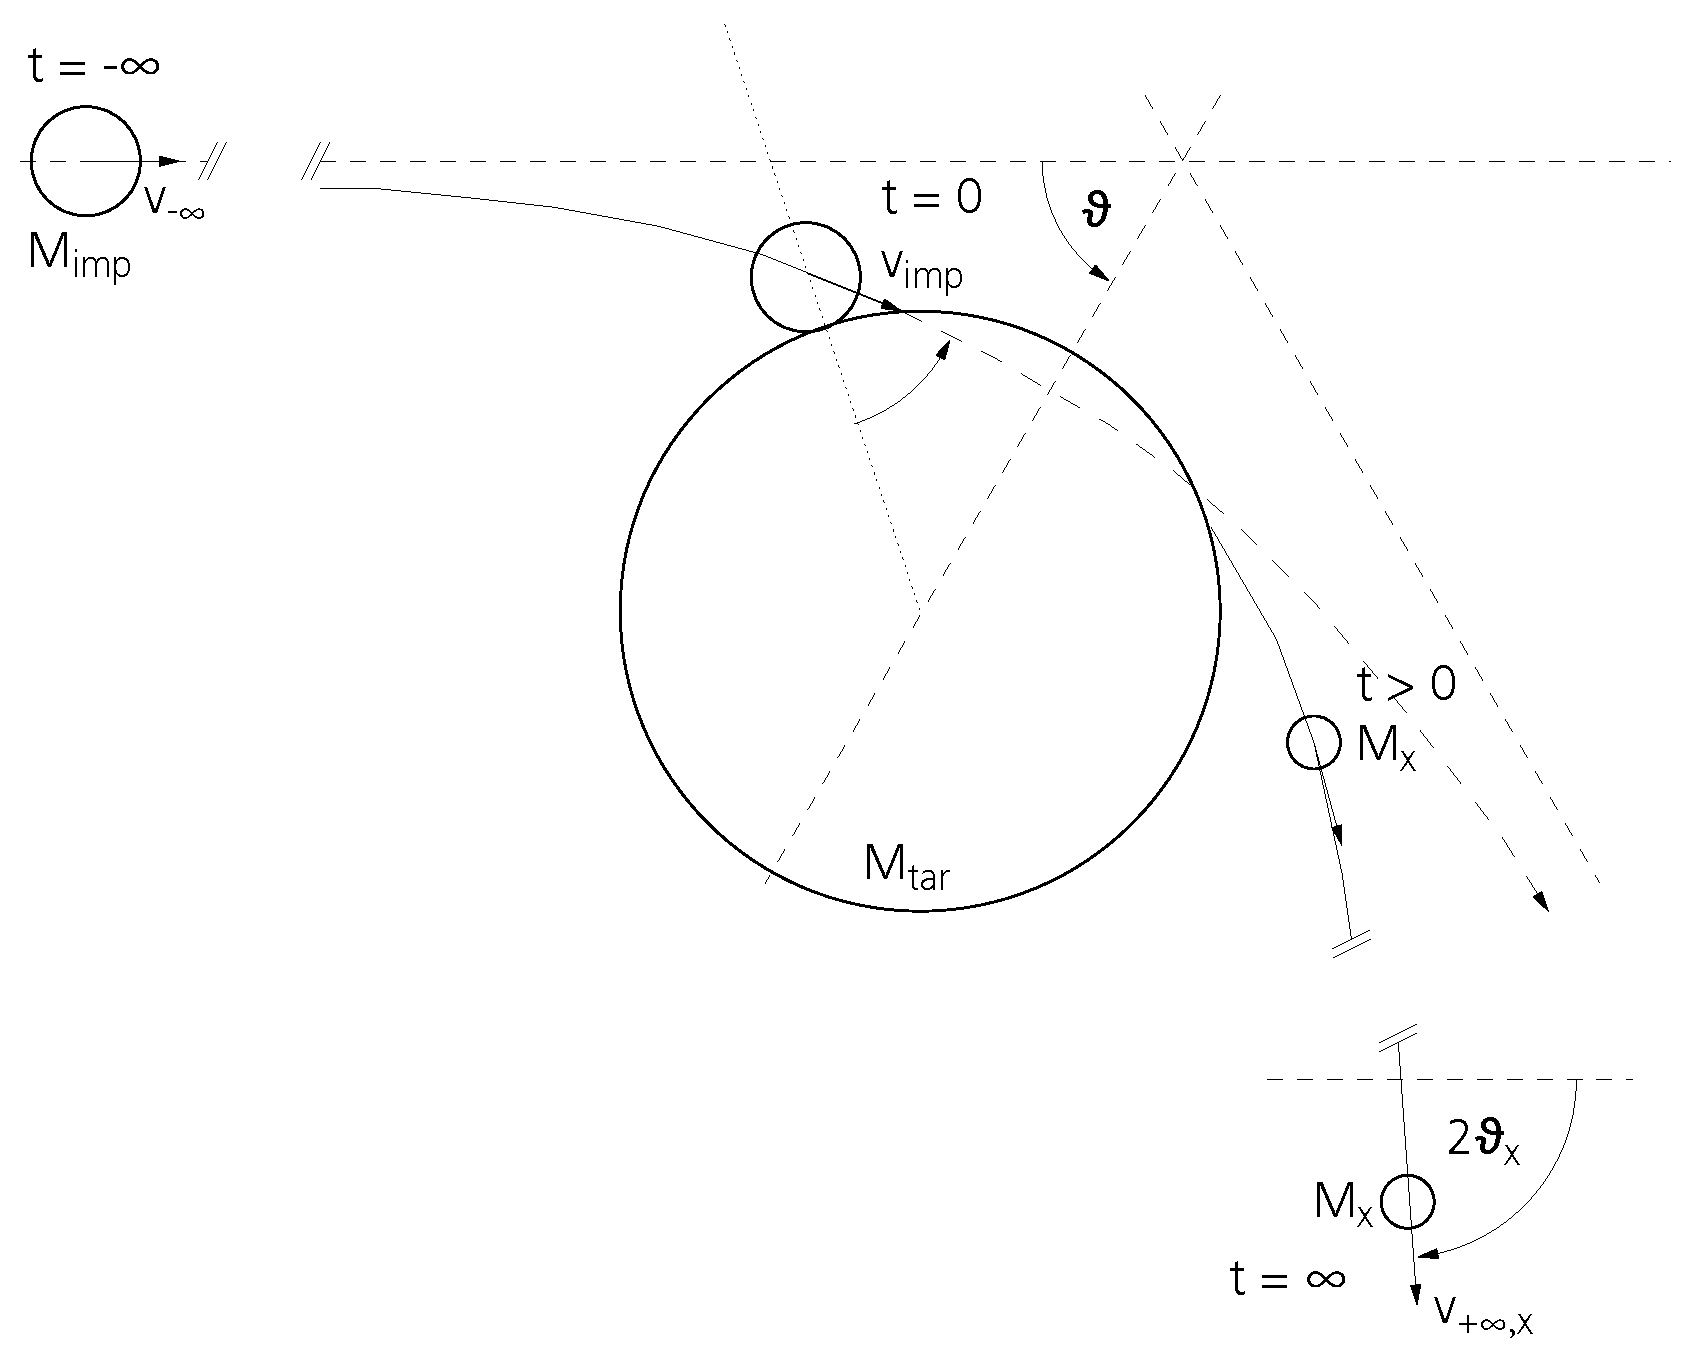
\includegraphics[scale=0.5]{04_vartheta}
\caption{Visualization of the deflection angle: The impactor approaches the target on a hyperbola (or on a parabola in case of $\vinf = 0$). Without a collision the total deflection angle of the impactor would be simply $2 \vartheta$.}
\label{ch03_fig02}
\end{center}
\end{figure}

\begin{landscape}

\begin{figure}[htbp]
\begin{center}
\includegraphics[scale=1.0]{21_SR_vinf_c1.pdf}
\caption{Relative velocity between the largest remnant and the second remnant at infinity as a function of impact angle for the simultion set \emph{c1}.}
\label{ch03_fig21a}
\end{center}
\end{figure}

\begin{figure}[htbp]
\begin{center}
\includegraphics[scale=1.0]{21_SR_vinf_i1.pdf}
\caption{Relative velocity between the largest remnant and the second remnant at infinity as a function of impact angle for the simultion set \emph{i1}.}
\label{ch03_fig21b}
\end{center}
\end{figure}

\begin{figure}[htbp]
\begin{center}
\includegraphics[scale=1.0]{22_SR_vartheta_c1.pdf}
\caption{Difference between the actual deflection angle of the second remnant and the expected deflection angle $2 \vartheta_{orb}$ for the impactor assuming an orbit of two point masses as a function of impact angle for simulation set \emph{c1}. Only points }
\label{ch03_fig22a}
\end{center}
\end{figure}

\begin{figure}[htbp]
\begin{center}
\includegraphics[scale=1.0]{22_SR_vartheta_i1.pdf}
\caption{Difference between the actual deflection angle of the second remnant and the expected deflection angle $2 \vartheta_{orb}$ for the impactor assuming an orbit of two point masses as a function of impact angle for simulation set \emph{i1}}
\label{ch03_fig22b}
\end{center}
\end{figure}
\end{landscape}


%%
% ejecta 
%% 
\subsection{Ejecta}
cite Lisse\\
analyze ejecta, entropy and energy of ejecta \\
show decay of shock wave plot\\ % TODOPLOT

\begin{landscape}
\begin{figure}
\begin{center}
\includegraphics[scale=1.0]{20_ejecta_r3.pdf}
\caption{Mass averaged mean disk eccentricities for the largest remnant disk as a function of impact angle for different impact velocities in the \emph{r3} simulation set. Simulations with a largest remnant disk mass below $0.1\% M_tot$ are omitted.}
\label{ch03_fig20a}
\end{center}
\end{figure}

\begin{figure}
\begin{center}
\includegraphics[scale=1.0]{20_ejecta_c1.pdf}
\caption{Mass averaged mean disk eccentricities for the largest remnant disk as a function of impact angle for different impact velocities in the \emph{r3} simulation set. Simulations with a largest remnant disk mass below $0.1\% M_tot$ are omitted.}
\label{ch03_fig20b}
\end{center}
\end{figure}

\begin{figure}
\begin{center}
\includegraphics[scale=1.0]{20_ejecta_i1.pdf}
\caption{Mass averaged mean disk eccentricities for the largest remnant disk as a function of impact angle for different impact velocities in the \emph{r3} simulation set. Simulations with a largest remnant disk mass below $0.1\% M_tot$ are omitted.}
\label{ch03_fig20c}
\end{center}
\end{figure}
\end{landscape}



\section{Discussion}
little toy model population in the early solar system (-> chambers) \\
% TODO: a little estimate for a toy model population in the early solar system: take 4 different sized bodies and analyze collisions into each other. make a plot with transition probabilities?

discuss topics in the light of the results. for example for Moon formation

\begin{figure}[htbp]
\begin{center}
\includegraphics[scale=0.7]{06_vimp}
\caption{An order of magnitude estimation of the random velocities for bodies undergoing collisions in a protoplanetary system with a solar mass central star. The random velocity is roughly the Kepler velocity times the orbital eccentricity. Shown are isolines of velocities for given distance from a star with a solar mass for given eccentricities. The red line shows the speed of sound of for quartz at standard conditions \cite{Melosh:2007p3502}. Note that the actual impact velocity is given by $\vimp = \sqrt{ v_{rand}^2 + \vesc^2}$ and depends on the masses of the two colliding bodies. Due to the high Kepler velocity in the inner parts of the system, even small eccentricities lead to random velocities well above the speed of sound for silicates and therefore to hypervelocity impacts even for small bodies.}
\label{ch03_fig06}
\end{center}
\end{figure}






	
\cite{Agnor:2004p3329}
%Agnor \& Asphaug 2004: accretion efficiency during planetary collisions
%- impact probability of eps: dP = 2*sin(eps)*cos(eps)*deps (Shoemaker 1962)
%- non-disruption doesn't mean merging
%- M1: largest remnant, M2: largest escaping remnant
%- M2 / Mesc < 0.8 for 30deg -> chains
%- two 0.1Mearth mass bodies, chondritic, Tillotson
%- non-accretionary collisions are the norm

\cite{Asphaug:2006p3729}
%Asphaug 2006: h\&r planetary collisions
%- 0deg: shocks dominate, 90deg gravity (tides, stresses) dominates
%- "strings of pearls"
%- for large bodies, the impactor, not the target, are destroyed
%- tidal vs. self-gravity stress inversely proportional to mass
%- relativ energy deposition 

\cite{Asphaug:2010p3539}
%Asphaug 2010: SSC collisions and the diversity of planets
%- next-largest bodies (NLB)
%- hit&run common for v_rand = v_inf
%- Safronov number 1-2 in late systems
%- SSC: contact compression timescale  (2r/v_imp) on gravity timescale ( r*sqrt(G*rho) )
%- shear stress exceeds strength above 100km
%- turn-around the target reference frame: the impactor is the altered body
%- Agnor 1999: angular momentum easily above dynamical stability
%- SSC scale-invariant to the first order
%- 45deg as the median impact angle (Shoemaker 1962)
%- small r/R -> impact cratering
%- "grazing": center of impactor skims tangential to the target
%- impact cratering: angle gives all or nothing, SSC is a continuum
%- for r_core = 0.5*r -> 30deg to 90deg miss each others cores
%- h&r prevalent for NLB
%- NLBs get mantle-stripped
%- tidal disruption important for small bodies
%- icy collision might be similar to rocky ones (ice : rock ~ rock : iron)
%- iron-enriched fragments from chain-events
%- h&r happen to about half the NLB?


\cite{2009ApJ...700L.118M}
%Marcus 2009:
%- confirmation of Stewart & Leinhardt 2009 for bodies > 100km
%- masses 1., 5., 10. Mearth, ratios 0.25, 0.50, 0.75
%- scaling relationship for MFe / Mlr
%- compositional changes require: a) small impact angle or b) small & fast impactor

\cite{2010ApJ...712L..73M}
%Marcus et al. 2010: Minimum radii from Super-Earths: Constraints from GIs
%- super-Mercuries are not expected, as striping bodies would have to be > 10 MEarth

\cite{2010ApJ...714L..21K}
%Kokubo \& Genda 2010:
%- about half the collisions do not accrete
%- orbit integration of 16 bodies, total mass 2.3MEarth
%- mass ratios: 1.0, 0.66, 0.50, 0.33, 0.25, 0.17, 0.11, Mtot = 0.2-2.0MEarth
%- impact velocities: 1.0-3.0 v_esc, angles: 0-75deg
%- criteria for critical impact velocity v_cr / v_esc for which accretion occurs
%- critical spin angular velocity

\cite{2011arXiv1105.4616E}
%Elser et al, 2011:
%- Moon formation in planetary systems
%- might be crucial for life

\cite{Chambers:2001p2105}
\citep{chandrasekhar1969ellipsoidal}
\cite{Lissauer:1993p56}
\cite{Wetherill:1993p3351}


\bibliographystyle{plainnat}
\bibliography{bibliography}



